% !TEX root = ../../my-thesis.tex
%
\graphicspath{{./content/introduction/figures/}}

\chapter{Introduction}

\cleanchapterquote{Nature loves to hide.}{Heraclitus (c. 6th-5th century BCE)}{}


\label{chap:intro}

\section{Context}

\subsection{Ecological and economic systems as complex adaptive systems}

What are the similarities between the dynamics of ecological and economic systems? 
% 
Think of an ecological system as a community of interacting biological organisms \citep{chapin2002principles}, and think of an economic system as a community of interacting economic agents \citep{Dopfer2007}.
% 
The dynamics of an ecological system depend on fluxes of matter and energy between organisms, and the dynamics of an economic system depend on fluxes of capital between economic agents.
% 
\textit{A priori}, the underlying processes strongly differ, because the behavior of economic agents is motivated by rationality, where economic agents maximize utility \citep{10.1093/cje/bet027}. 
% 
Nonetheless, economic agents are faced with uncertainty \citep{Foster2012} and their rationality is bounded \citep{Veblen1898,nelson1985evolutionary}. As a result, economic agents adopt a variety of behavioral rules \citep{Foster2012} through trial-and-errors, which are themselves subject to natural selection through competition processes \citep{schumpeter2017theory}.
% 
Along this perspective, both ecological and economic systems are complex adaptive systems \citep{Levin2002}, composed of heterogeneous entities that interact in nonlinear ways and experience evolutionary processes. 
% 
% Interaction and evolutionnary processes take many different forms and operate at different organizational level \citep{Levin1998} (see \cref{fig:organisational_levels}).
% 
The processes of interaction and evolution involved operate at different organizational level \citep{Levin1998}, from genes to ecological communities, and from individual behavior rules to economies, and affect each other across the organizational levels through different coupling (see \cref{fig:organisational_levels}).
% 
Interestingly, the stochasticity of the processes at stake, and their couplings, do not necessarily lead to unpredictable structures and dynamics, but rather induce organized structural properties and invariant patterns \citep{Olff2009,mitchell2009complexity}. 
% 
In ecological systems, invariant patterns include, for instance, patterns of species richness, where e.g. montane regions are often associated with a disproportionately high number of species \citep{Rahbek2019}. In economic systems, invariant patterns include, for instance, the bimodal shape of the distribution of international income, where some countries have systematically developed much more rapidly than others \citep{acemoglu2001colonial}. 
% 
A common direction on the research agenda in biology and economics is to understand general organizational principles, i.e.  to underpin the fundamental processes and couplings that generate invariant patterns \citep{Levin2002,Olff2009,Veldhuis2018}.
% 
In ecological systems, the fundamental processes resulting affecting biodiversity are identified \citep{Rahbek2019a,Rangel2018,Hagen2022}, and the current challenge is to underpin the mechanisms resulting from their couplings \citep{Hagen2022}.
% 
In economic systems, we still do not exactly understand the fundamental processes at stake. 


%% Figure parallels
\begin{figure}[ht]
    \centering
    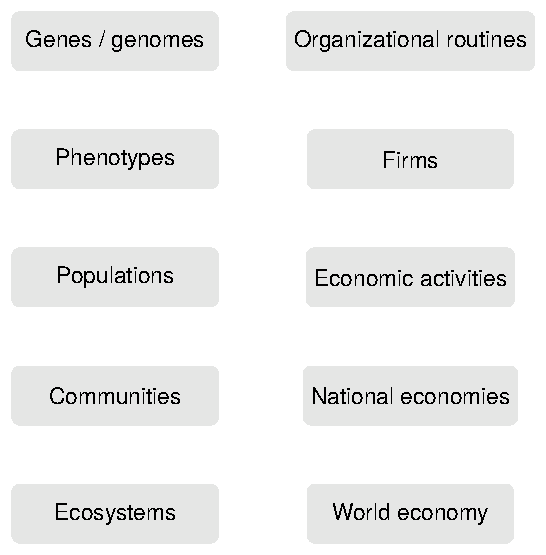
\includegraphics{organizational_complexity.pdf}
\caption{\textbf{Graphical representation of organizational levels and their couplings in ecological and economic systems}. An arrow indicates that the organizational level at its tail can influence the organizational level at its head. Left diagram is inspired from \cite{Hendry+2016}.}
\label{fig:organisational_levels}
\end{figure}

\subsection{Ecological and evolutionary processes drive the dynamics of ecological systems}
 
In ecological systems, interaction processes are more commonly designated as ecological processes, and encompass the processes of interaction between organisms (biotic interactions) and between organisms and their environment (abiotic interactions), as well as dispersal processes (movement of individual across space) (\cite{Vellend2010a}, see \cref{fig:eco_evo} for a graphical representation).
% 
Evolutionary processes designate those processes responsible for the change of heritable characteristics (DNA, genes, phenotypes) over successive generations (\cite{Hall2013}, \cref{fig:eco_evo}).
% 
The coupling between ecological and evolutionary processes is acknowledged since the very birth of the theory of evolution. 
% 
During his voyage on the Beagle, Darwin documented a link between the different ecological opportunities across the Galápagos Islands and the different beak shapes in the finches he found on each island \citep{darwin2004origin}.
% 
He reasoned that the variations in ecological opportunities lead to a differential in survival for certain phenotypes, which over time resulted in the evolution of different beak shapes.
% 
Since then, we know that ecological processes interact with evolutionary processes, and they together shape the long term dynamics of ecological systems \citep{Urban2016,Rahbek2019a,Rangel2018,Hagen2022}.

%%
Empirical studies have now demonstrated that evolution can be rapid and occur on similar time scales as ecology \citep{Hairston2005, Pelletier2009}. This coupling has quantifiable effects on ecological dynamics \citep{Ezard2009}, leading to feedbacks between ecological and evolutionary processes, so-called eco-evolutionary feedbacks \citep{Pelletier2009,Schoener2011,Govaert2019}. 
% 
% Example of eco-evolutionary dynamics
Eco-evolutionary feedbacks involve situations where an ecological process (e.g., replication, competition, dispersal) influences an evolutionary process (e.g. phenotypic change), which then feeds back to an ecological process, or vice versa (\cite{Govaert2019}, \cref{fig:eco_evo}). Examples are feedbacks between population dynamics (replication and competition) and phenotypic change, which can lead to evolutionary branching through the effect of competition \citep{Dieckmann1999}.
% 
In spatially structured populations, another classical example of eco-evolutionary feedbacks is the mechanism of local adaptation \citep{Savolainen2007}, where feedbacks between population dynamics, dispersal and trait evolution can facilitate or prevent populations to adapt to local environmental conditions \citep{Meszena1997,Doebeli2003}.
% 
Importantly, the eco-evolutionary feedbacks involved in adaptation mechanisms are expected to affect the dynamics of ecosystems in the coming decades \citep{Norberg2012,Urban2016}, because of the expected rapid changes in environmental conditions due to anthropogenic pressure and climate change \citep{Ellis2011,Midgley2019}.
% 
Nevertheless, our understanding of eco-evolutionary feedbacks in realistic ecological scenarios is limited \citep{Lion2022}.

\begin{figure}[ht]
    \centering
    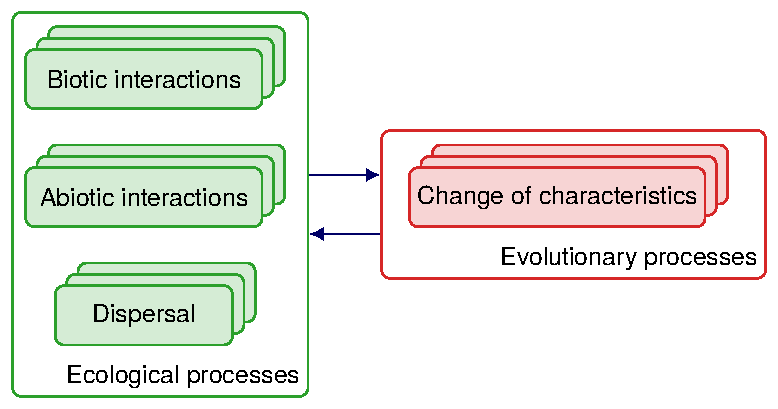
\includegraphics{eco_evo.pdf}
\caption{\textbf{Graphical representation of the eco-evolutionary processes determining eco-evolutionary dynamics in ecological systems.} By extension, I use this terminology to designate interaction and evolutionary processes in economic systems.}
\label{fig:eco_evo}
\end{figure}

\subsection{Drivers of economic change}

In economic systems, the fundamental processes determining economic change are controversial \citep{Dopfer2007,Nelson2014,Hodgson2019}. 
%
To explain economic change, Neoclassical theory \citep{10.1093/cje/bet027} assumes that economic systems are in equilibrium, in the sense that the demand and supply of goods and services are balanced on all relevant markets. 
% 
Firms are rational in maximizing profits by adapting to demand and supply, and the observed economic change is driven by exogenous forces, such as technological innovations \citep{Romer1986}. Evolutionary economics, promoted by the seminal work of \cite{Nelson2014}, criticizes this view and seeks to explain economic change by focusing on endogenous forces. 
% 
%% Foundations of evolutionary economics
Evolutionary economics suggests that eco-evolutionary processes, acting upon firms and their organizational routines, are major processes contributing to economic change \citep{Hodgson2019}.
% 
Organizational routines designate the ensemble of behavioral or technological rules that define the cohesive identity of the firms, and play the same roles as genes, defining how firms engage in interactions with other firms, and experiencing evolutionary processes \citep{nelson1985evolutionary}. Firms being elemental units of economic systems \cite{nelson1985evolutionary}, through couplings across the different organizational levels, these eco-evolutionary processes should affect economic change at the local, regional, national, and international scale (see \cref{fig:organisational_levels}).

%%
The deep analogy between genes and organizational routines, together with the subsequent analogies between firms and phenotypes, between economic activities and biological populations, and between the processes acting upon them, (\cref{fig:organisational_levels}), invite understanding economic change with biological concepts.
% 
Accordingly, a number of modelling approaches have borrowed concepts and methods from biology, aiming at underpinning the fundamental processes underlying invariant patterns in economic systems \citep{Tacchella2018,Saavedra2009a,Scholl2020,Zhang2018,Modis1997,Saavedra2014,Farmer1999,Michalakelis2011,Marasco2016,Gatabazi2019,Cauwels56,Applegate2021,Suweis2015}. 
% 
For instance, \cite{Saavedra2009a} has successfully used a model of mutualistic interaction to explain structural patterns in industrial cooperation.
% 
Also, \cite{Scholl2020} uses the concepts of food webs and population dynamics to explain market malfunctions and excess volatility in financial markets.
% 
However, those studies did not seek to understand how eco-evolutionary processes may affect economic change at the national scale.
% 
Biologically inspired eco-evolutionary models may help to disentangle the effect of eco-evolutionary processes on the dynamics of national economic systems, and could explain differences in economic change across countries.

\section{Modeling eco-evolutionary dynamics}

\subsection{Forward modelling of eco-evolutionary processes}
The complex interplay between ecological and evolutionary processes can hardly be studied with experimental approaches (\cite{Pontarp2019,Hagen2022}, but see \cite{Becks2012} for an experimental study with rotifer-alga microcosms). 
% TODO: cite \citep{May2004}
As such, deductive reasoning, relying on forward modelling, has traditionally been put forward to underpin the mechanisms underlying invariant patterns in ecological systems \citep{Brummitt2020}. Along this approach, hypotheses about causal processes are embedded in a model, whose simulation (forward integration) generates predictions (see \cref{fig:forward_inverse_modelling}). A fundamental aspect of forward modelling is to underpin the underlying mechanisms, i.e. to disentangle how the interplay between the processes generate the predictions. 
% 
%% early mathematical models
In the early 1930s to 1940s, by formulating tractable mathematical models implementing the processes of reproduction, dispersal and mutations, the work of Fisher, Wright and Haldane has greatly contributed to the modern synthesis of evolutionary biology \citep{huxley1942evolution}, generally accepted as the basis of our current understanding of evolutionary dynamics. 
% 
Yet in order to obtain tractable mathematical model, Fisher, Wright and Haldane have neglected eco-evolutionary feedbacks \citep{Govaert2019}. In particular, their works have relied on strong simplifications concerning the ecological processes, and have neglected the effect of evolutionary processes on population dynamics \citep{Lion2022}.

%% computers
With the increase in computational capacity, novel modelling approaches relying on individual-based models have appeared \citep{deangelis2005individual}. These models require less simplifying assumptions than traditional mathematical models \citep{deangelis2005individual}, and can unveil more realistic mechanisms by allowing to capture processes acting at the individual level. However, the lack of analytical tractability of individual-based models is a shortcoming, because it challenges the ability of the modeler to underpin general principles from the simulations \citep{Lion2016,May2004}.
% 
%% computers and analytical framework
The recent development of mathematical techniques, such as moment closure approximations \citep{law1999moment,Gandhi2000,Nordbotten2020,Lion2016}, adaptive dynamics theory \citep{Metz1995}, and probability theory \citep{Champagnat2006}, are generating novel pathways by filling the gap between individual-based models and mathematical models. 
% 
Analogous to renormalization group analysis developed in quantum and statistical physics \citep{Sayama}, they form a toolbox to rigorously identify the couplings across the organizational levels. As such, these mathematical techniques allow an analytical underpinning to individual-based model simulations, and can generate a general understanding of the key mechanisms at stake \citep{Lion2016}.

%% examples of the combination of computer models and analytical tools
The combination of numerical simulations and, e.g., adaptive dynamics theory, has successfully shed light on the emergence of evolutionary branching under feedbacks between population dynamics and phenotypic change \citep{Dieckmann1999,Doebeli2003}.
%
Another example is the work of \cite{Meszena1997,Debarre2013, Mirrahimi2020}, that has provided new insights on the effect of habitat heterogeneity on local adaptation. 
% 
However, our current understanding of eco-evolutionary feedbacks neglects specificities of real biological populations that may significantly alter the resulting mechanisms, such as the organization of populations over complex spatial structures \citep{Nowak2001a} and highly dimensional phenotypic space \citep{Doebeli2010}.

% 
Investigating whether the features of realistic spatial and phenotypic structures affect eco-evolutionary feedbacks is important to advance our understanding, but raises challenging methodological issues. 
% 
In particular, the consideration of complex spatial structures may hinder the underpinning of general eco-evolutionary mechanisms in structured populations.
% 
Also, the consideration of multiple traits leads to an increase in the dimensionality of the models, which in turn leads to an exponential increase in the computational cost associated with the numerical simulations \citep{Bellman1957}.
% 
In order to advance our understanding of eco-evolutionary dynamics, we need to understand how the features of realistic spatial and phenotypic structures affect eco-evolutionary feedbacks, which in turn requires methodological developments, in order to cope with the extra complexity and computational cost.

\begin{figure}[t]
    \centering
    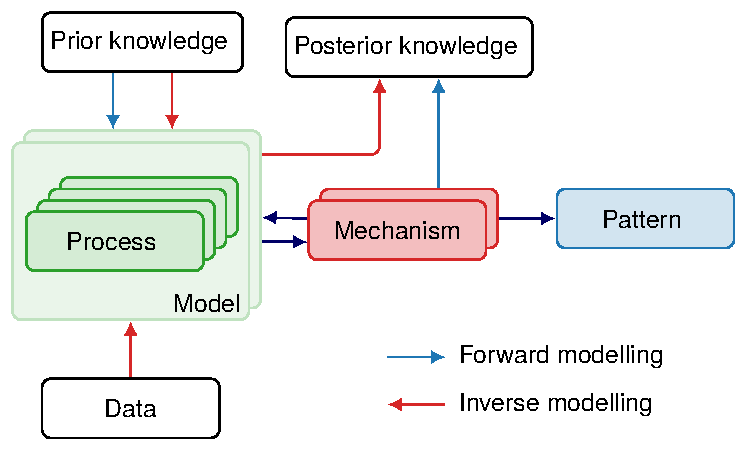
\includegraphics{forward_inverse_modelling.pdf}
    \caption{\textbf{Forward and inverse modelling approaches for the understanding of complex adaptive systems}. A forward modelling approach consists in deriving a model, embedding a set of processes inspired from prior knowledge. The objective is to understand how the interplay between the processes considered transforms in (feedback) mechanisms that are associated with a prediction. An inverse modelling approach integrates empirical observation within the modelling process. Posterior knowledge on the empirical system is obtained whether form the interpretation of the estimated parameter values, or through model selection.
    }
    \label{fig:forward_inverse_modelling}
\end{figure}

\subsection{Inverse modelling}
%% inverse modelling
Another approach to underpin processes and mechanisms in ecological systems consists in inverse modelling, where empirical data is used to constrain the model (\cite{Clermont2015}, see \cref{fig:forward_inverse_modelling} for a graphical illustration).
% 
Inverse modelling can take the form of parameter estimation \citep{Schartau2017} or model selection \citep{Johnson2004}, both involving the use of inference methods to estimate the probability of the empirical data given the model parameters (i.e., the likelihood).
% 
Provided that they are inferred together with uncertainties, parameters can be interpreted to better understand the strengths and effects of the processes considered \citep{Pontarp2019}. For instance, \cite{Higgins2010,Curtsdotter2019} infer the parameters of population dynamic models to understand the processes involved in ecosystem functions.
%
In model selection, candidate models embedding competing hypotheses about causal processes are derived, and the relative support of each model given the data is computed to discriminate between the hypotheses \citep{Johnson2004}. For instance, using inverse modelling and eco-evolutionary models embedding competing evolutionary speed hypotheses, \citep{Skeels2022} shows that temperature-dependent evolutionary speed most likely explains variations in biodiversity patterns.

The computation of the most probable model parameter values, or the computation of the different model supports, critically involves inference methods.
% 
Inference methods commonly demand many forward integration of the model, resulting in a computational cost that can be prohibitively expensive \citep{Schneider2017}.
% 
The number of forward integration required may dramatically increase with the number of model parameters \citep{Csillery2010}, and the number of model parameters, together with the model nonlinearities, can eventually lead to false estimates of the most probable model parameter values \citep{Gabor2015}.
% 
Consequently, inverse modelling methods have mostly been used with simple evolutionary models \citep{Csillery2010}. 
% 
Eco-evolutionary models are dependent on numerous parameters \citep{Boyd2012}, are strongly nonlinear \citep{Hastings1993,Huisman1999,Beninca2008}, and their integration is computationally expensive \citep{Fisher2018}, challenging the use of inverse modelling to underpin eco-evolutionary processes. 
% 
Advances in the field of artificial intelligence could circumvent these issues, allowing to advance our knowledge of eco-evolutionary dynamics in empirical systems.  

\subsection{Artificial intelligence to leverage forward and inverse modelling}

\label{subsec:artificial intelligence}
In the recent years, the field of artificial intelligence has made enormous progresses in computer vision \citep{voulodimos2018deep} and natural language processing \citep{young2018recent}. At the backbone of this success are key computational techniques that could leverage the forward and inverse modelling of eco-evolutionary dynamics.
% 
Advances in computer vision and natural language processing rely on deep learning methods, that allow neural networks to learn abstract representation of mechanisms from large datasets \citep{LeCun2015}.
% 
These abstractions can hardly be interpreted to generate scientific theories \citep{Karpatne2017}, and their prediction ability is limited by the information contained in the training datasets. As such, neural networks cannot be used \textit{per se} to gain scientific insights and extrapolate beyond observed trends \citep{Barnosky2012,Urban2016}.
% 
Nevertheless, their traditional applications and associated methods have been successfully derived in other scientific fields for this purpose \citep{Kashinath2021,Schneider2017,Yazdani2020,Rolnick2023}.
%
%% ML for forward modelling
For instance, neural networks have been used to reduce the cost of the forward integration of climate models, learning more efficient representations of physical mechanisms \citep{Kashinath2021}.
% 
They have also been used to approximate the solution of partial differential equation (PDE) models \citep{Sirignano2018dgm,Han2018}, with the major advantage of approximating high dimensional problems at a lower computational cost than traditional methods.
% 
Beyond accelerating model simulations, \cite{Rackauckas2020a} suggests that advances in artificial intelligence can be used to infer scientific knowledge. The authors argue that generalized variants of the backpropagation algorithm -- used for the training of neural network \citep{LeCun2015}-- can be used to train any scientific model against data \citep{Rackauckas2020}, with the potential to leverage inverse modelling techniques \citep{Frank2022}. 
% 
Together, artificial intelligence techniques may offer unique opportunities for advancing our understanding of eco-evolutionary dynamics, but require a profound shift in the scientific programming paradigm.


\subsection{Scientific programming and computational environments}

\label{subsec:Julia}
Combining artificial intelligence techniques with scientific models requires a computational environment that allows to easily develop scientific models, while ensuring simulation performance, and providing composability between artificial intelligence and other scientific libraries \citep{Rackauckas2020}. Unfortunately, performance and composability are features that are poorly represented in mainstream programming languages used by the scientific community, such as Python, Matlab or R.
% 
%% performance and ease of use
Those languages are naturally attractive because they are dynamically typed \citep{Bezanson2017}, allowing convenient development iterations. Nonetheless, prototypes written in Python, Matlab or R need to be rewritten in low level, compiled languages such as C, C++ or Fortran for speed and predictable mapping to hardware \citep{Perkel2019,Bezanson2017}. This conversion requires significant efforts, leading to a problem commonly designated as the "two-language problem" \citep{Bezanson2017}.
% 
In order to circumvent performance issues, most libraries in Python, Matlab or R rely on bindings with low level languages. For instance, the most used deep learning libraries in Python, TensorFlow and PyTorch, are internally written in C++ (see \cite{tensorflow,pytorch}). However, bindings with low level languages come with major negative externalities. First, they restrict the understandability of their source code to computer scientists -- prohibiting potential development contributions from the scientific community. Second, they prevent the composability of, e.g., traditional scientific computing libraries and deep learning libraries \citep{Innes2019}. This absence of composability arises because to be trained, numerical models must be differentiated with respect to their parameters. Yet, deep learning libraries such as TensorFlow or PyTorch are only able to differentiate models written in their own internal source code \citep{Innes2019}.

%% Julia 
Julia is a recently developed programming language that addresses the issue of the two-language problem \citep{Bezanson2017,Bezanson2018}. Julia was built over a type-specializing, just-in-time compiler, which makes it easy to generate performant programs in pure Julia, while preserving the essential features of Python, Matlab or R, such as dynamic typing and automatic memory management \citep{Perkel2019}. 
% 
The source code of most Julia libraries is consequently written in pure Julia, guaranteeing understandability and composability.
% 
In particular, Julia is an automatic differentiation pervasive language \citep{Innes2019}, which allows to differentiate any model written in pure Julia without any modification. As a result, deep learning libraries can be used on any scientific model written in Julia \citep{Rackauckas2020a}.
% 
Solving the two-language problem, Julia permits scientists to prototype a program which is readily generic and performant, benefitting not only the development process but also the entire research community \citep{Bezanson2017}.
% 
Overall, the composability and productivity granted by Julia makes it an ideal computational environment to accelerate research. 

\section{Thesis outline}

In summary, while it is increasingly acknowledged that feedbacks between ecological and evolutionary processes play an important role in ecological systems \citep{Pelletier2009, Urban2016}, our understanding of eco-evolutionary dynamics in biological populations structured in realistic phenotypic and geographic space is limited \citep{Lion2016,LiebermanHauert2005,Doebeli2011}.
% 
Under increasing anthropogenic pressure, advancing this understanding is essential \citep{Urban2016} but raises challenging methodological issues.
% 
Further, while analogous processes to eco-evolutionary processes have been suggested to influence the dynamics of economic systems \citep{Hodgson2019}, we do not know their effect on economic dynamics at the scale of a country.
% 
Here, I develop novel forward and inverse modelling methods, that I use to shed light on general eco-evolutionary processes and feedbacks shaping the dynamics of ecological and economic systems.


In \cref{chap:diff-in-graphs}, I investigate how eco-evolutionary processes, in combination with complex habitat structures, influence the phenotypic distribution of biological populations. 
I proceed using a forward modelling approach: I derive a stochastic eco-evolutionary individual-based model where individuals are structured over a spatial graph, and experience the fundamental processes of reproduction, competition, mutation and migration. Seeking to understand how those processes result in phenotypic differentiation at the population level, I derive analytical approximations of the individual-based model. Together with extensive numerical simulations, they provide insights into how the graph properties affect the population size and phenotypic differentiation. In particular, I show that three main graph properties, relating to landscape connectivity, heterogeneity in connectivity, and habitat spatial auto-correlation, shape phenotypic differentiation. These results establish mechanistic links between landscape features and the eco-evolutionary dynamics of biological populations.

In \cref{chap:mini-batching}, I develop an inverse modelling method to estimate the parameters of eco-evolutionary models and perform model selection. The method is based on a machine learning framework and involves the combination of state-of-the-art artificial intelligence techniques and a novel learning strategy. The learning strategy consists in training the model against mini-batches of data with short time horizon, which I analytically show to solve convergence problems arising from model nonlinearities. I implement the ML framework in a new Julia library released under the name of \textbf{MiniBatchInference.jl}, and demonstrate through numerical experiments that it can efficiently and accurately estimate model parameters and provide model support from noisy, incomplete and independent time series. Altogether, the proposed ML framework is a workhorse for inverse modelling and can elucidate mechanistic pathways in ecological and economic systems.

In \cref{chap:econobiology}, I quantify the effect of eco-evolutionary processes on the dynamics of economic systems. I employ the ML framework developed in \cref{chap:mini-batching} to investigate how alternative eco-evolutionary population models can explain the dynamics of economic activities in 77 of the world's richest countries, relying on 59 year of economic data. The models embed processes acting upon economic activities, including ecological interactions between them, their spatial dispersal, and their transformations. The statistical support of each model is compared to a simple logistic growth model, taken as a null model. I find strong statistical evidence for positive interactions and spatial dispersal. To my knowledge, this is the first study providing quantitative evidences that eco-evolutionary processes shape the dynamics of economic systems at the country level.

In \cref{chap:nonlocalPDE}, I extend two recent methods to solve high dimensional non-local nonlinear PDEs. This class of PDEs can be used to construct generic eco-evolutionary models of biological populations structured over complex phenotypic spaces, but up to now, could only be simulated in low dimensions. The first method presented relies on Picard iterations, while the second is based on deep learning and involves neural networks to approximate the PDE model simulations. I implement both methods in a new Julia library released under the name of \textbf{HighDimPDE.jl}, and evaluate their performance on high dimensional eco-evolutionary PDE models, and on PDE models arising in physics. The methods yield good results with short run times, opening up new venues to further our understanding of eco-evolutionary dynamics in realistic populations.

\newpage
